%
% BUS 338: Foundations of Innovation - A Course Overview
%
% Author: Jeffrey Leung
%

\documentclass[10pt, oneside, letterpaper, titlepage]{article}

\usepackage[ampersand]{easylist}
	\ListProperties(
		Progressive*=5ex,
		Space=5pt,
		Space*=5pt,
		Style1*=\textbullet\ \ ,
		Style2*=\begin{normalfont}\begin{bfseries}\textendash\end{bfseries}\end{normalfont} \ \ ,
		Style3*=\textasteriskcentered\ \ ,
		Style4*=\begin{normalfont}\begin{bfseries}\textperiodcentered\end{bfseries}\end{normalfont}\ \ ,
		Style5*=\textbullet\ \ ,
		Style6*=\begin{normalfont}\begin{bfseries}\textendash\end{bfseries}\end{normalfont}\ \ ,
		Style7*=\textasteriskcentered\ \ ,
		Style8*=\begin{normalfont}\begin{bfseries}\textperiodcentered\end{bfseries}\end{normalfont}\ \ ,
		Hide1=1,
		Hide2=2,
		Hide3=3,
		Hide4=4,
		Hide5=5,
		Hide6=6,
		Hide7=7,
		Hide8=8 )
\usepackage{geometry}
	\geometry{margin=1.2in}
\usepackage{graphicx}
	\graphicspath{ {img/} }
\usepackage[colorlinks=true, linkcolor=blue]{hyperref}
\usepackage{graphicx}
	\graphicspath{ {./img/} }
\usepackage{lmodern} % Allows the use of symbols in font size 10; http://ctan.org/pkg/lm
\usepackage{pdfpages}
\usepackage{textcomp} % Allows the use of \textbullet with the font
\usepackage{verbatim}

\renewcommand{\arraystretch}{1.2}
\renewcommand{\familydefault}{\sfdefault}

\title{BUS 338: Foundations of Innovation \\\medskip \Large A Course Overview}
\author{Jeffrey Leung \\ Simon Fraser University}
\date{Summer 2018}

\begin{document}

	\maketitle
	\tableofcontents
	\clearpage

	%
% CMPT 213: Object Oriented Design in Java - A Course Overview
% Section: Introduction
%
% Author: Jeffrey Leung
%

\section{Introduction}
	\label{sec:introduction}
\begin{easylist}

& Standards:
	&& Make fields private when possible

& Commenting:
	&& Comment purpose of a class
	&& Name fields/methods/parameters so comments are unnecessary

& When possible, convert strings to non-string types internally for consistency

& \textbf{Clean code:} Code which is correct, easy to read/maintain, and conforms to a standard

& Software design:
	&& 4 steps:
		&&& Requirements
		&&& Design and implementation
		&&& Verification
		&&& Evolution
	&& Designing involves identifying classes, responsibilities, and relationships to create a diagram
	&& Implementation process options:
		&&& \textbf{Skeleton code:} Beginning minimal parts/features of a system
		&&& \textbf{Component-wise:} Creating components one at a time
	&& Methods of integrating code from multiple people:
		&&& \textbf{Continual integration:} Gradual system growth by constantly integrating changes
		&&& \textbf{Big Bang integration:} Building all parts separately without integrating until the end

& \textbf{Feature envy:} Characteristic of a class which relies heavily on another class
& Warning sign: Characteristic of a method which operates more strongly on another object than its own
& \textbf{Deprecation:} State where a public interface is no longer supported or recommended, and is slated to be removed in the future


& \textbf{try-catch:} Structure which watches for an exception and handles it
	&& Only one exception can be live at a given time
	&& \textbf{finally clause:} Optional clause after catch clauses which is executed regardless of the result
		&&& If exception is thrown, the finally clause is executed immediately afterwards
	&& \textbf{try-with-resources:} Block which cleans up a resource when a try block exits

& Exception: Issue which may be fixable and is not out of the software's control
	&& \textbf{Checked exception:} Exception which must be caught or listed in a throws clause
	&& \textbf{Unchecked exception:} Exception which will automatically propagate and does not require catching
		&&& E.g. RuntimeException
		&&& Preferred as it does not require modification of methods between try/catch, which decouples code

\end{easylist}
\clearpage

	%
% BUS 338: Foundations of Innovation - A Course Overview
% Section: Marketing
%
% Author: Jeffrey Leung
%

\section{Marketing}
	\label{sec:marketing}
\subsection{Markets and Segments}
	\label{subsec:markets-and-segments}
\begin{easylist}

& \textbf{Marketing:} Strategy and process of identifying, targeting, engaging, and acquiring customers

& \textbf{Market:} Set of consumers who have similar perceptions and preferences, have specific needs and desires fulfilled by a set of products or services, and who reference each other when making a buying decision
	&& Types of market:
		&&& \textbf{Clone market:} Consumers who will buy into a copy of an existing business model
		&&& \textbf{Existing market:} Consumers who will purchase a higher-end product which is faster, more efficient, etc.
		&&& \textbf{Cheaper segmented existing market:} Consumers who will purchase a lower-end product
		&&& \textbf{Niche segmented existing market:} Consumers who will purchase a product with distinct marketing/branding
		&&& \textbf{New market:} Consumers in a unique new class grouped by a new factor
	&& Characteristics of a market:
		&&& Customers: Needs/pain points, adoption details
		&&& Nature of the market: Size, entry cost, competitive barriers
		&&& Sales margins
		&&& Time to profitability

& Learn about markets by researching:
	&& Government statistics
	&& Industry sources and reports
	&& Companies currently in the industry
	&& People you know from the industry
	&& Interviews/surveys/focus groups with current customers, lead users, field experts

& \textbf{Market segment:} Group of consumers who have common needs and desires who can be targeted by their common perceptions, preferences, and drives, and can reference each other in the buying decision process
	&& Possible segmentation factors: Product usage, demographics, psychographics (personality, values, interests, lifestyle), geography
	&& Segment based on the customers' perceived value, buying process, and behaviours
	&& Do not segment based on demographics, unknown internal behaviours, competitors' segmentation
	&& Process of segmentation: Document market sizing details, determine scoring criteria, determine segment attractiveness, choose initial target segment, select market targets
	&& Characteristics of a segment: End user, needs, urgency of needs, benefit, lead customer, willingness to change/adapt, cost of entry, frequency of buying, size of market, competitive barriers, type of market (clone, resegmented, existing, new)
	&& \textbf{Beachhead segment:} Market segment which is the initial domination target by a product
		&&& Should be small enough to dominate, large enough to have an impact, and be strategically aligned with the product's strengths and weaknesses

& \textbf{Sales-driven marketing:} Positioning of a product to attract any buyer regardless of their characteristic
	&& Initially more attractive than market-driven because of the immediate interest
	&& Eventually will fail and lead to low sales
& \textbf{Market-driven marketing:} Positioning of a product to attract only buyers with specific characteristics
	&& More effective than market-driven because of the ability to dominate a market segment and create cohesive references between buyers

\end{easylist}
\subsection{Positioning Statements and Value propositions}
	\label{subsec:positioning-value}
\begin{easylist}

& \textbf{Positioning:} Portrayal of a product in the mind of the consumer by the company, through marketing in contrast to the competitors
	&& Focuses on customer needs/pains, value of the product, and differentiation from competing products
	&& One positioning statement per target market segment, and one positioning statement for the entire market
	&& Composition of a positioning statement:
		&&& For \textit{target customers} \\
		Who need \textit{compelling reason to buy} \\
		Our product is a \textit{new product category} \\
		That provides \textit{key problem-solving capability; addresses the reason to buy}. \\
		Unlike \textit{competitors' alternative products}, \\
		Our product \textit{key product features and differentiation}. \\
		We also provide \textit{other parts of the product}.

& Types of buyers:
	&& Each target market has a unique set of buyers
	&& \textbf{User buyers}: Group of people who will be using the product or managing the users (i.e. end-users)
	&& \textbf{Technical buyers}: Group of people who do not choose the product, but must approve the purchase (e.g. finance department, regulators, parents)
	&& \textbf{Economic buyers}: Group of people who have the ability to pay for the product (e.g. CEO, CFO, management team, parents)

& \textbf{Value proposition:} Statement about the product's benefits to a specific group of buyers
	&& Varies per audience (one per buyer type per market, and one for each other player in the market - e.g. influencers)
	&& Composition of a value proposition:
		&&& We believe that \textit{target customers} \\
		Should be able to \textit{ability to address need} \\
		By \textit{specific measurement or KPI \#, \$, \%} \\
		Through the ability to \textit{key problem-solving capability; addresses the reason to buy} \\
		As a result of \textit{key product features and differentiation} \\
		For an investment of approximately \textit{\$ estimate}.
	&& Examples:
		&&& \textit{User buyer:} We believe that transfusion nurses \\
		Should be able to reduce transfusion labour \\
		By 75\% \\
		Through the ability to eliminate the 2\textsuperscript{nd} nurse checker and simplify the transfusion process \\
		As a result of implementing barcode cross-checking at the bedside \\
		For an investment of approximately \$200,000.
		&&& \textit{User manager buyer:} We believe that hospital blood bank managers \\
		Should be able to reduce blood bank labour \\
		By 30\% while maintaining existing service levels \\
		Through the ability to allocate blood just-in-time rather than in advance \\
		As a result of implementing on-demand blood issuing \\
		For an investment of approximately \$200,000.
		&&& \textit{Economic buyer:} We believe that hospital CFOs \\
		Should be able to reduce the overall cost of blood transfusions \\
		By 10\% \\
		Through the ability to eliminate wasted blood products and reduce blood inventory levels \\
		As a result of introducing blood tracking and on-demand blood issuing \\
		For an investment of approximately \$200,000.

\end{easylist}
\subsection{Market Adoption Cycle}
	\label{subsec:market-adoption-cycle}
\begin{easylist}

& \textbf{Market Adoption Cycle:} Segmentation of potential buyers by their willingness to adopt an innovation
	&& See figure~\ref{fig:market-adoption-cycle}

\begin{figure}[!htb]
	\centering
	\caption{Market Adoption Cycle}
	\label{fig:market-adoption-cycle}
	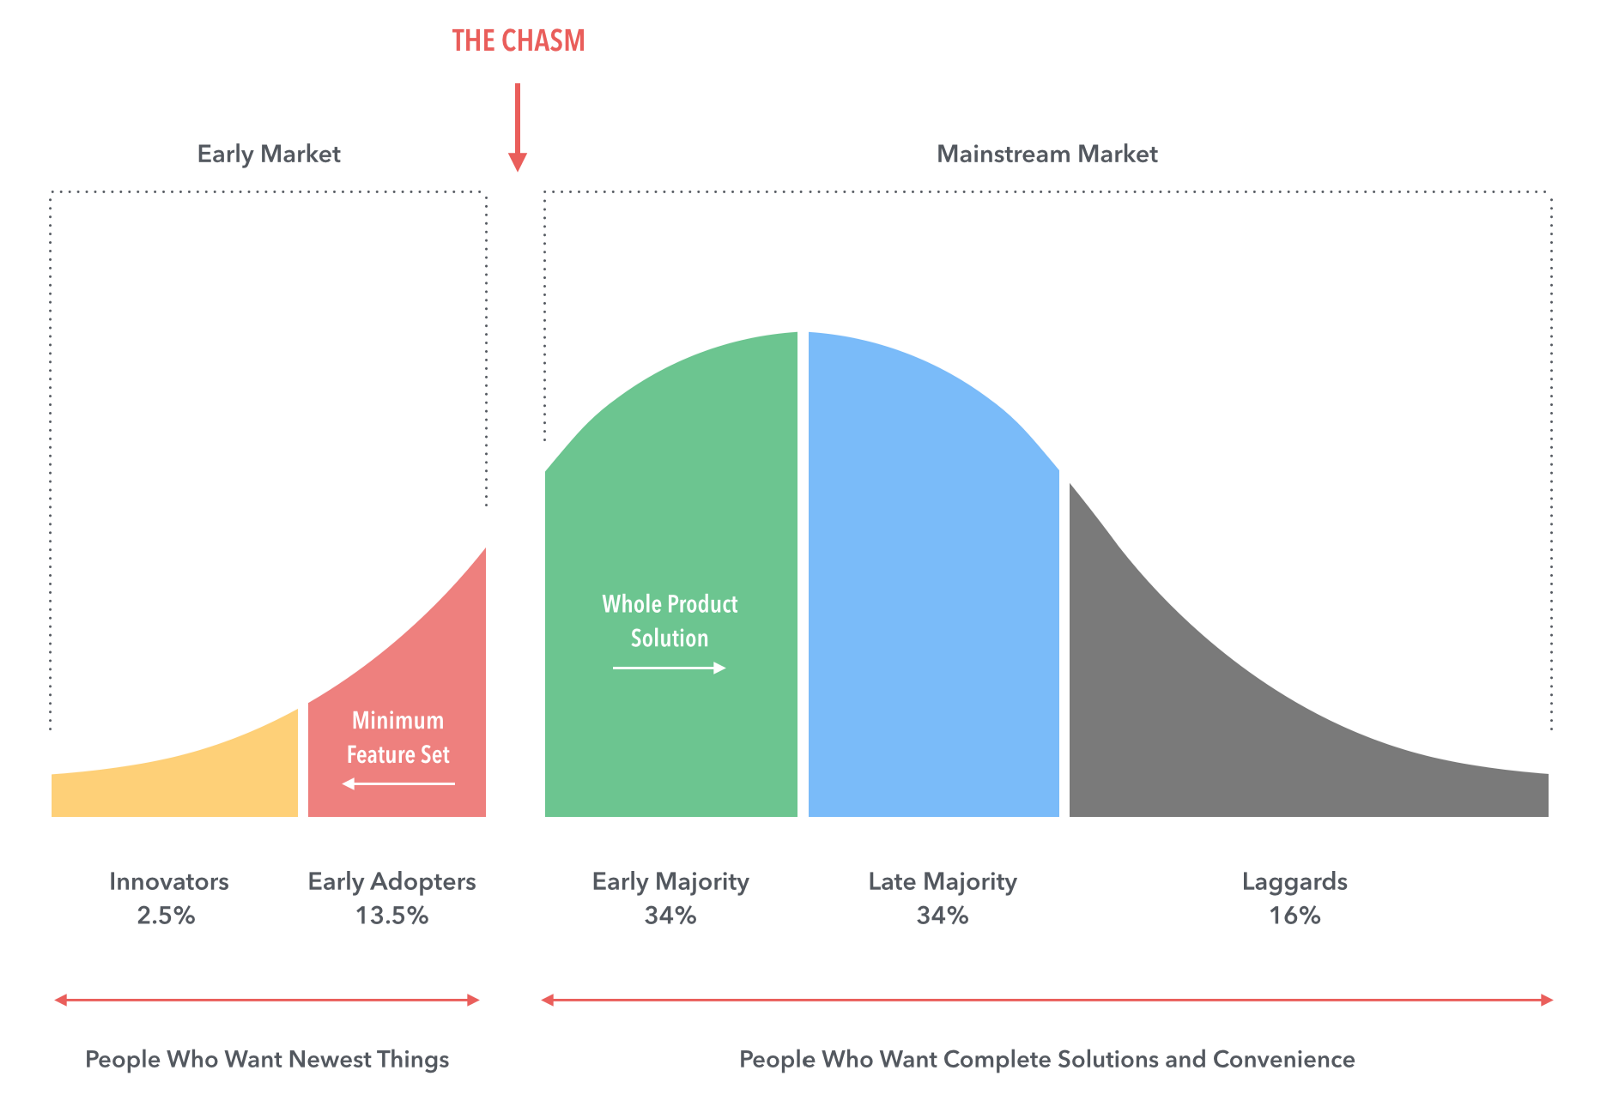
\includegraphics[width=0.7\textwidth]{market-adoption-cycle}
\end{figure}

& \textbf{Innovators:} Enthusiast buyers who actively seek out new innovations
	&& Innovation for the sake of innovation
	&& Desire to be early buyers
	&& Forgiving of and willing to work to resolve problems
& \textbf{Early adopters:} Visionary buyers who use intuition to choose innovations for their own needs
	&& Willing to buy in early
	&& Expectations of significant change from existing solutions
	&& Not price-sensitive
& \textbf{Early majority:} Pragmatist buyers who buy technologies which are proven by market leaders
	&& Larger population
	&& Highly practical
	&& Expectations of incremental change from existing solutions
	&& Require a complete solution
& \textbf{Late majority:} Comfortable buyers who only buy products which are easy to use and safe against decay over time
	&& Larger population
	&& Need support
	&& Need the market to already be dominated by the product
& \textbf{Laggards:} Reluctant buyers who dislike new innovations and will only buy technology which is absolutely necessary

& Characteristics of adopting an innovation:
	&& Relative advantage over existing offerings
	&& Visible and easily understandable value and use
	&& Ease of use when moving from an existing offering
	&& Compatibility with pre-existing conditions and environmental factors

\end{easylist}
\subsection{Pitching}
	\label{subsec:pitching}
\begin{easylist}

& Structure of a pitch:
	\begin{enumerate}
		\item Introductions
		\item The problem and those who experience it
		\item Impact of the problem
		\item Current situation and solutions
		\item Our solution and its desired outcome
		\item Solution's benefits (not features/details)
		\item Competitors
		\item Unique positioning/differentiator and how it benefits the user
		\item Where we have an advantage
		\item Make an ask
	\end{enumerate}

\end{easylist}
\clearpage
	%
% BUS 338: Foundations of Innovation - A Course Overview
% Section: Product
%
% Author: Jeffrey Leung
%

\section{Product}
	\label{sec:product}
\begin{easylist}

& \textbf{Whole product:} Basic product in addition to other factors which create a reason to buy or augment the basic product
	&& E.g. Installation, configuration, integration, maintenance, customer support, other compatible products
	&& Composed of several layered perceptions (see figure~\ref{fig:whole-product})
		&&& \textbf{Generic product:} Basic product provided to customer with no additional features
			&&&& E.g. Wardrobe as individual pieces
		&&& \textbf{Expected product:} Basic product with features which the customer assumes they will receive
			&&&& E.g. Wardrobe pre-built or with a worker to assemble it
		&&& \textbf{Augmented product:} Product with all features included to maximize the value provided to the customer
			&&&& E.g. Wardrobe delivered to the house and assembled by the worker, with a warranty
		&&& \textbf{Potential product:} Possibilities of additional features beyond the scope or abilities of the original product
			&&&& E.g. Wardrobe with built-in light and clothes categorization system
	&& Early adopters do not require a full product, but pragmatists often do

\begin{figure}[!htb]
	\centering
	\caption{Whole Product}
	\label{fig:whole-product}
	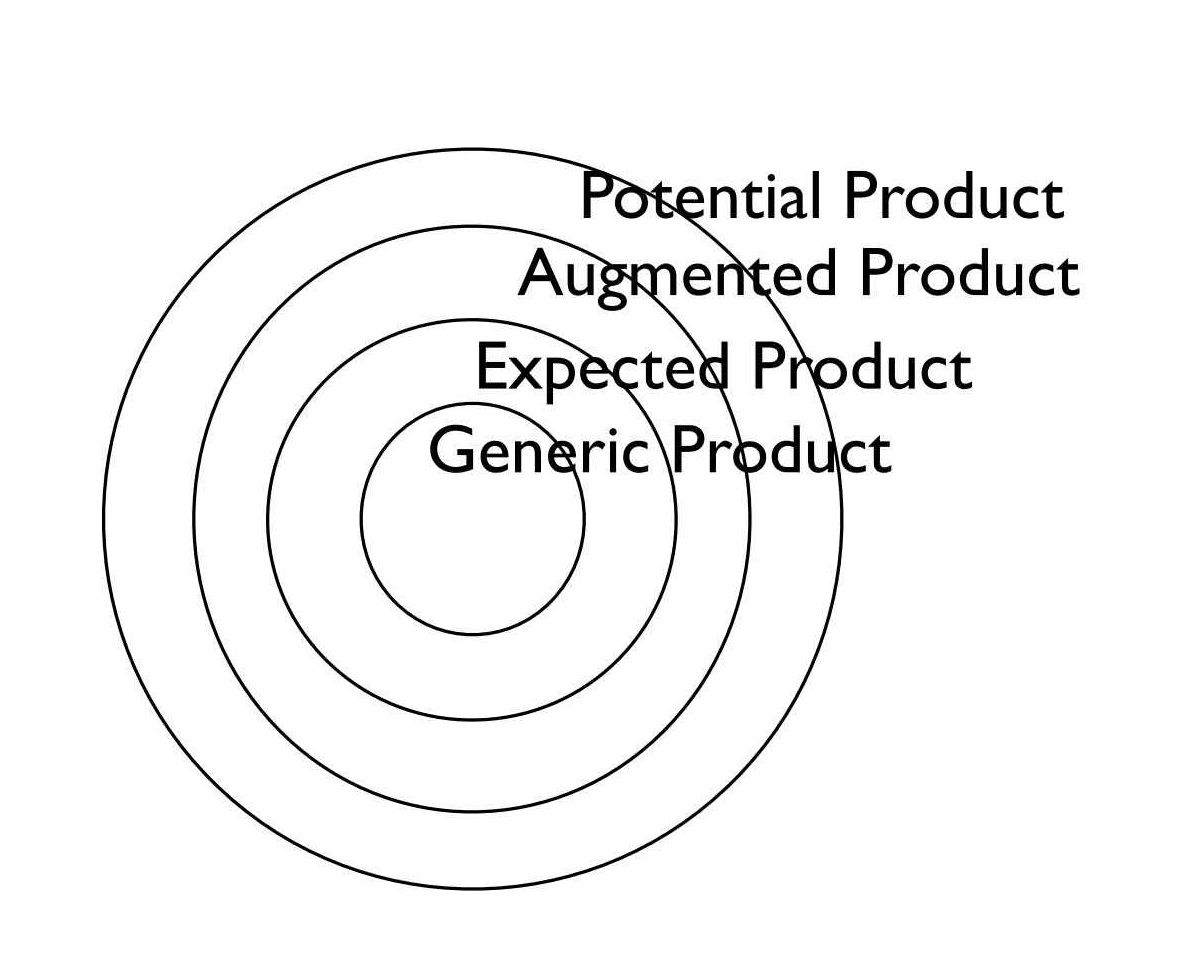
\includegraphics[width=0.7\textwidth]{whole-product}
\end{figure}

& Product characteristics:
	&& Features: Description, specifications, informative data (e.g. speed, dimensions, colors, models)
	&& Product benefits and key customer value: Reasons for using the solution and their importance (e.g. save time or money)
	&& Enhance the way that features add value to customers

& Match the prioritized customer needs to the product's benefits
	&& Needs must be important to the customer
	&& The match between benefits and needs should excel among the competition

\end{easylist}
\clearpage

	%
% BUS 338: Foundations of Innovation - A Course Overview
% Section: Research
%
% Author: Jeffrey Leung
%

\section{Research}
	\label{sec:research}
\begin{easylist}

& Gathering information qualitatively: Interviews, focus groups
& Gathering information quantitatively: Surveys, digital analytics

& When to research:
	&& Before devising a solution, research the problem and understand the customer
	&& While developing the solution, research its effectiveness and strategy

& When interviewing:
	&& Create hypotheses but be open-minded
	&& Choose research subjects based on specific common characteristics
	&& Do not sell a product or service
	&& Prefer face-to-face communication
	&& Pay attention to body language

& To communicate clearly:
	&& Contextualize the conversation
	&& Logically structure the message
	&& Focus on essential elements and their roles
	&& Remove ambiguous terms
	&& Use a style which engages the audience

\end{easylist}
\clearpage
	%
% BUS 338: Foundations of Innovation - A Course Overview
% Section: Competition
%
% Author: Jeffrey Leung
%

\section{Competition}
	\label{sec:competition}
\begin{easylist}

& \textbf{Competitor:} Company which has a product that, in the hands of a customer, decreases the value of your product
& \textbf{Complementor/partner:} Company which has a product that, in the hands of a customer in addition to your product, increases the value of your produc

& Alternative: Another company with the same market target
	&& Provides reference information on:
		&&& Price
		&&& Costs (sunk, running, and maintenance)
		&&& Promotion and distribution channels (current and potential)
		&&& How customers view the product
	&& Vital for pragmatists to compare against
	&& Important to position against
	&& \textbf{Market alternative:} Company currently servicing your prospective customers but which does not solve the problems you are strategically addressing
	&& \textbf{Product alternative:} Company is addressing the same problems as you and is vying for market leadership
	&& \textbf{Status quo:} Existing state without change

& Being the first to market is useful when:
	&& The product is difficult to duplicate
	&& The product satisfies customer needs well
	&& A significant proportion of the market can be quickly captured
	&& Obstacles for others can be created (e.g. regulations)

& Not being the first to market is useful when:
	&& A need is uncovered by an earlier company but not addressed
	&& Customer needs are unclear
	&& No dominant design has been accepted
	&& Switching costs are low

& Competition can be in the following factors:
	&& Brand
	&& Product attributes
	&& Quality
	&& Service
	&& Unmet needs of existing customers

& \textbf{Competitive matrix:} Analysis of customer interests addressed by your product or by competitors
	&& Categories should be accurate, actionable, and relevant
	&& Example categories:
		&&& Main customers
		&&& Key partners
		&&& Market share
		&&& Key products
		&&& Pricing
		&&& Key product features
		&&& Marketing channels
		&&& Sales channels
	&& See figure \ref{fig:competitive-matrix}

\end{easylist}

\begin{figure}[!htb]
	\centering
	\caption{Example of a Competitive Matrix}
	\label{fig:competitive-matrix}
	\begin{tabular}{ l | l l l }
		& Us & Competitor 1 & Competitor 2 \\
		\hline
		Main customers \\
		Key partners \\
		Key product features \\
		Pricing \\
		Sales channels
	\end{tabular}
\end{figure}

\clearpage

	%
% BUS 338: Foundations of Innovation - A Course Overview
% Section: User Experience
%
% Author: Jeffrey Leung
%

\section{User Experience}
	\label{sec:user-experience}
\subsection{Research and Insight}
	\label{subsec:user-experience:research-and-insight}
\begin{easylist}
	
& \textbf{User experience research:} Understanding the buyers/users and their needs and goals which can be supported by a solution
	&& Involves discarding initial assumptions
	&& \textbf{Problem research:} Understanding the identity of the buyers/users, their problems, and the context
	&& \textbf{Solution research:} Understanding the usability, feature set, and selling ability of a solution, and the customer satisfaction created

& \textbf{User insight:} Ability to understand the experience of users
	&& Can lead to an opportunity for new products, changes in communication/marketing, etc.
	&& Sources of insight:
		&&& Process of an experience
		&&& Division of labour
		&&& Unique combinations or usages of solutions
		&&& Benefits derived
		&&& Mistakes made
		&&& Frustrations
		&&& Ideal wishes perceived as unachievable
	
& \textbf{Ladder of inference:} Process by which user experience is understood more deeply and in context
\begin{enumerate}
	\item \textit{Observations and experiences} are perceived
	\item \textit{Filters} are applied to select pereceptions
	\item \textit{Meanings} are applied to add cultural and personal context
	\item \textit{Assumptions} are created based on meanings
	\item \textit{Conclusions} are drawn from assumptions
	\item \textit{Beliefs} are created about the subject and affect our future filters and meanings
	\item \textit{Actions} are taken based on beliefs and create new situations which are observed and experienced
\end{enumerate}

& Problems and solutions can be clustered in categories such as feelings, preferences, senses, places, communication, etc.

\end{easylist}
\subsection{Personas}
	\label{subsec:user-experience:personas}
\begin{easylist}

& \textbf{User persona:} Detailed overview of an ideal individual within a market segment, and their personality, preferences, and needs
	&& Criteria:
		&&& Basic demographics: Name, picture, age, gender
		&&& Background: Salary, household income, location, education, family
		&&& Job information: Company, company details (e.g. size, characteristics, main products), role in the company
		&&& Goals and challenges: Difficulties, ideals, current solutions
		&&& Values: Important factors, main objections, fears
	&& One persona for each type of buyer (user/technical/economic) and for anyone who is a part of the decision-making process (e.g. champions, influencers, veto powers)

\end{easylist}
\pagebreak
\subsection{Example Persona}
	\label{subsec:user-experience:example-persona}
\begin{easylist}

\begin{LARGE}
	\centerline{\textbf{Jim Davis}}
\end{LARGE}

\begin{figure}[!ht]
	\centering
	\label{fig:jim-davis}
	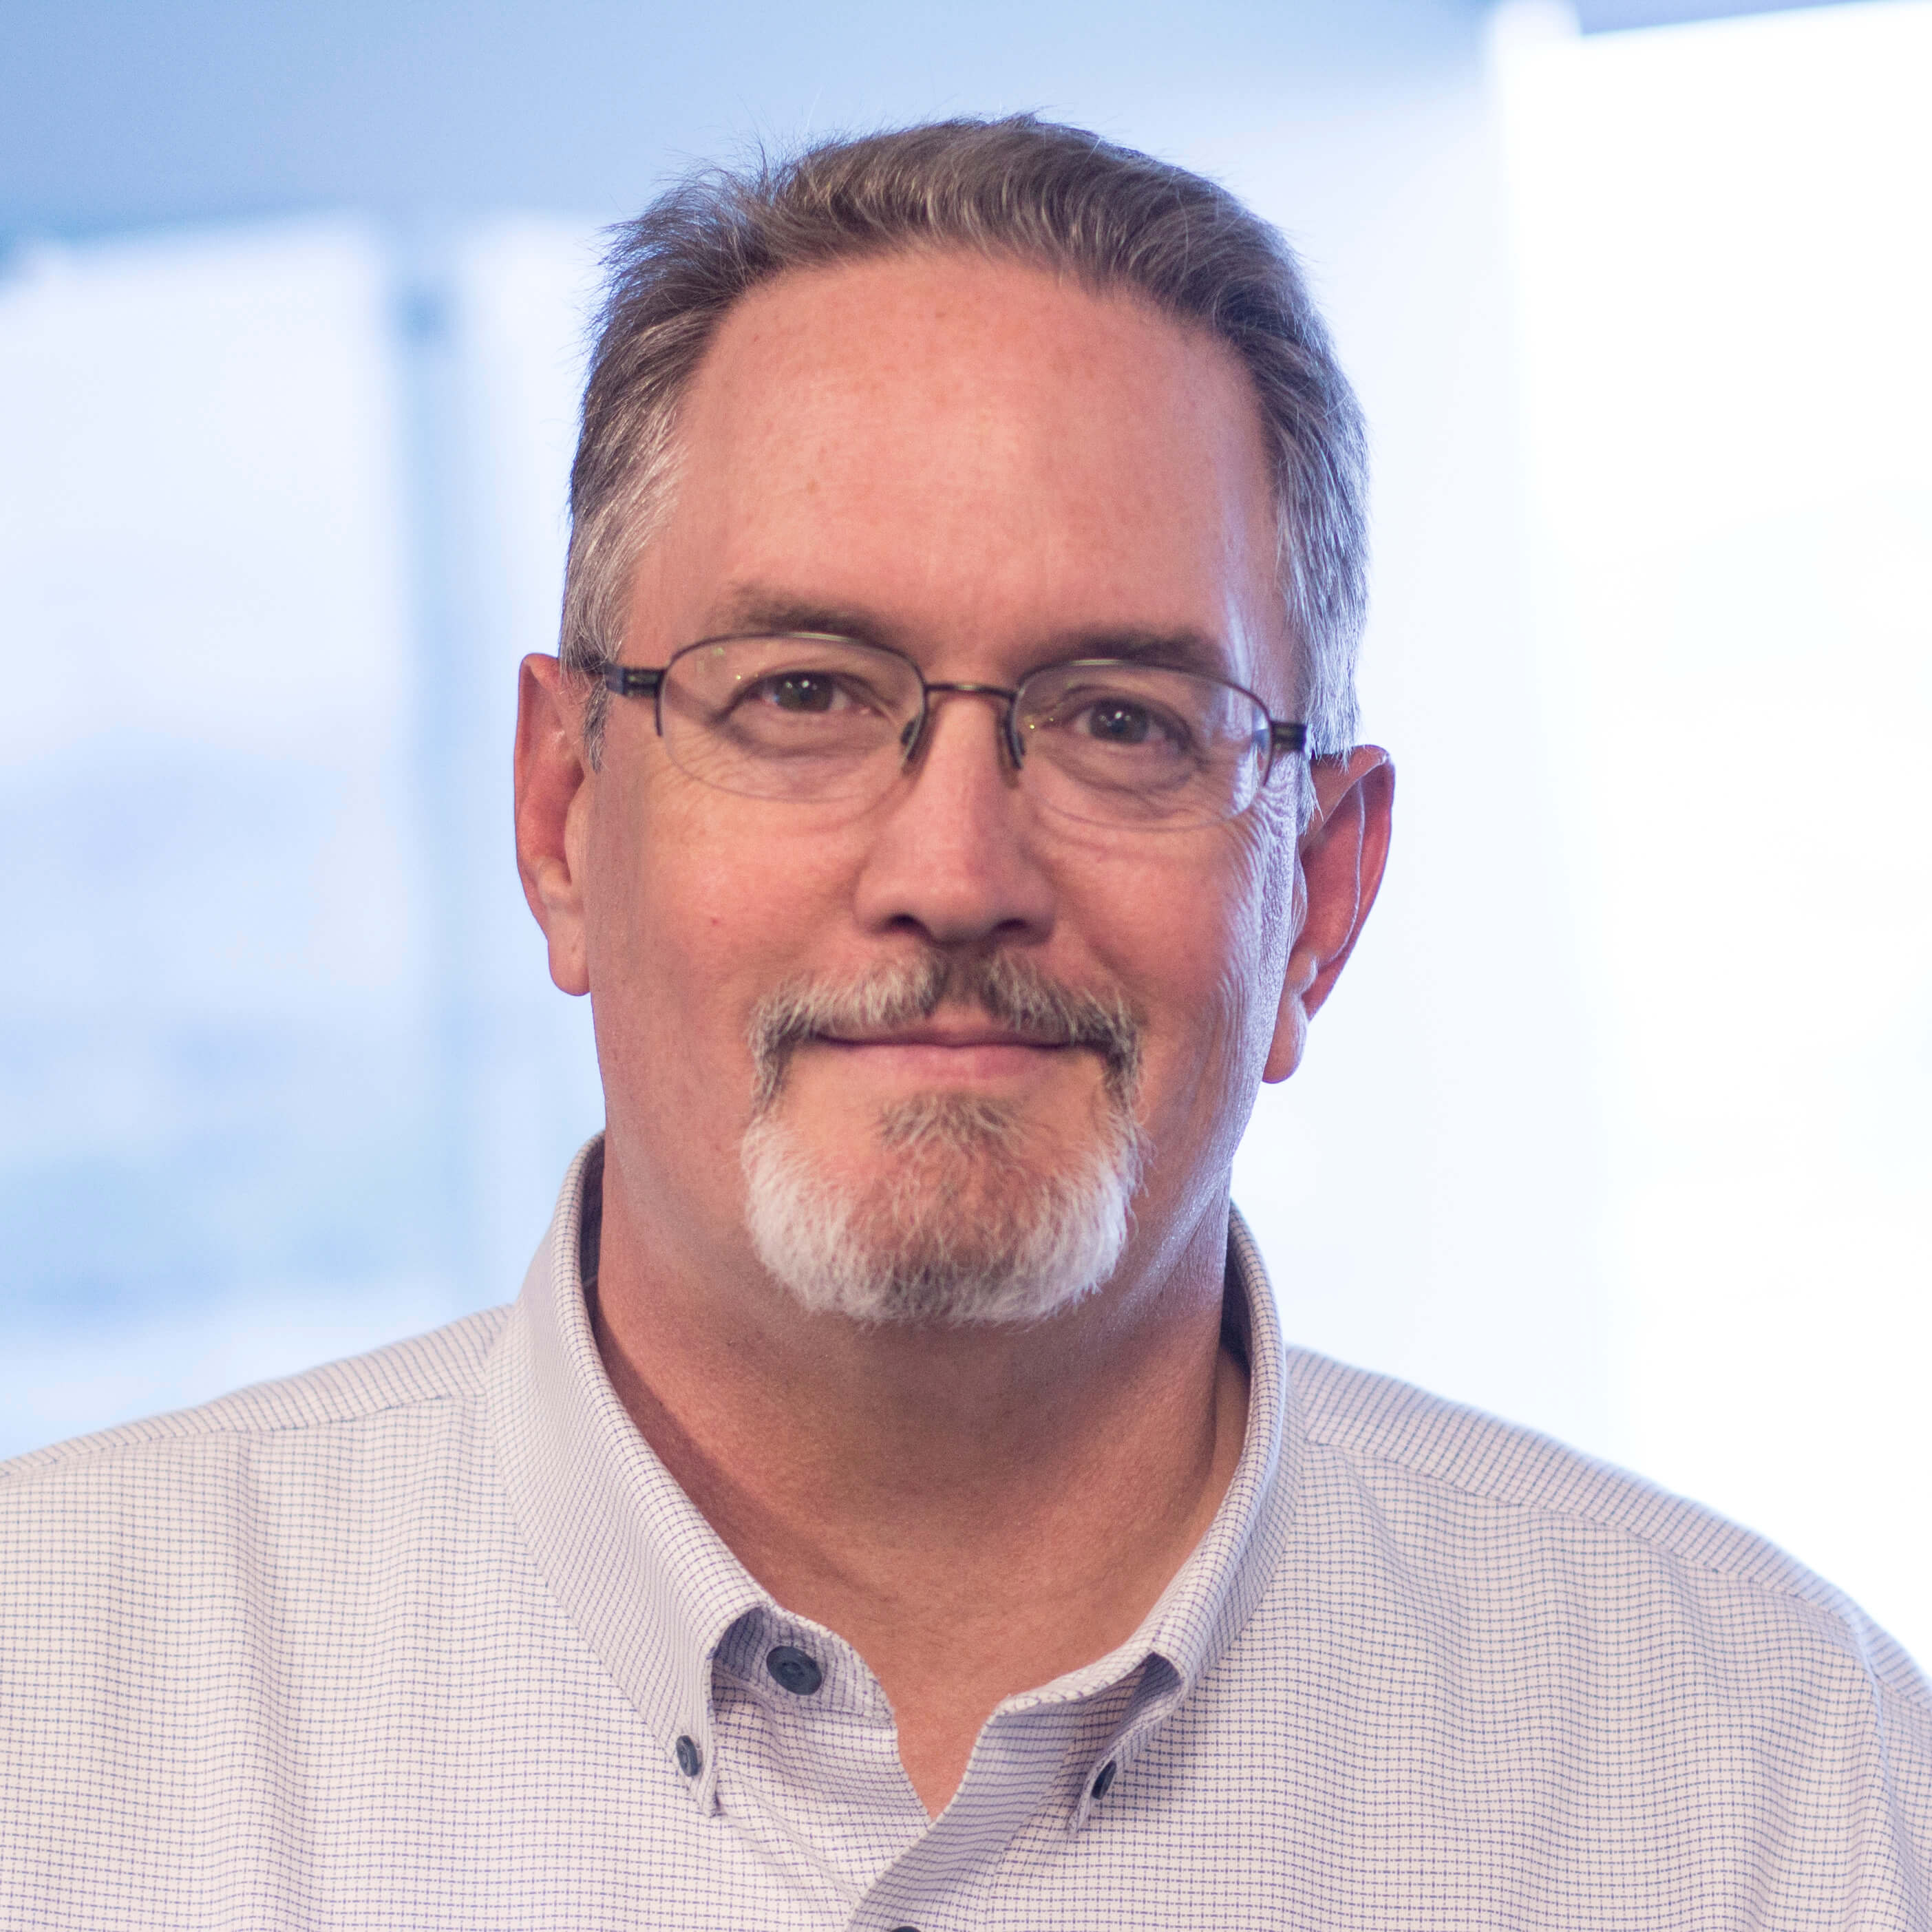
\includegraphics[width=0.4\textwidth]{jim-davis}
\end{figure}

\noindent
\textbf{Biography:} \\
48 years old \\
Married with children (high-school age) \\
Works at Siemens as a Project Manager
Ph.D in Computer Science from MIT \\
Has been managing teams for 15 years. Hands-on. Writes code frequently. \\
Drives a Toyota Prius \\
Carries a Samsung Note

\vspace{1em}

\noindent
\textbf{Behaviours:} \\
Reports to the General Manager \\
Manages the software organization and the associated budget \\
Makes all key decisions on tools and systems for the software organization

\vspace{1em}

\noindent
\textbf{Needs and Goals:} \\
Wants his team to create high-quality code \\
Willing to pay a premium price for the best tools to support his workers

\end{easylist}
\clearpage

	%
% BUS 338: Foundations of Innovation - A Course Overview
% Section: Innovation Ecosystem
%
% Author: Jeffrey Leung
%

\section{Innovation Ecosystem}
	\label{sec:innovation-ecosystem}
\begin{easylist}

& \textbf{Innovation ecosystem:}

& Consists of:
	&& The end customers
	&& Intermediaries
	&& Complementors
	&& Influencers
	&& Upstream suppliers of each component
	&& Competitors

& In addition, identify:
	&& The value provided by the product
	&& Risks at each step
	&& Ways around road blocks
	&& Standards and regulations (e.g. legalities, taxes, workplace, trading, marketing, environment, manufacturing)

& Every downstream group between you and the customer must receive value from you

& \textbf{Execution risk:} Challenges in developing an innovation to specification within time and resource limitations
& \textbf{Co-innovation risk:} How a commercialization depends on the success of another commercialization
	&& E.g. Smartphones require the successful development of many components
& \textbf{Adoption risk:} How partners need to adopt an innovation before end consumers can access your product
	&& E.g. Michelin Run Flat tires were adopted by every partner except for the repair shops which did not carry the component

\end{easylist}
\clearpage

	%
% BUS 338: Foundations of Innovation - A Course Overview
% Section: Appendices
%
% Author: Jeffrey Leung
%

\section{Appendix A: Business Model Canvas}
	\label{sec:appendix-a}

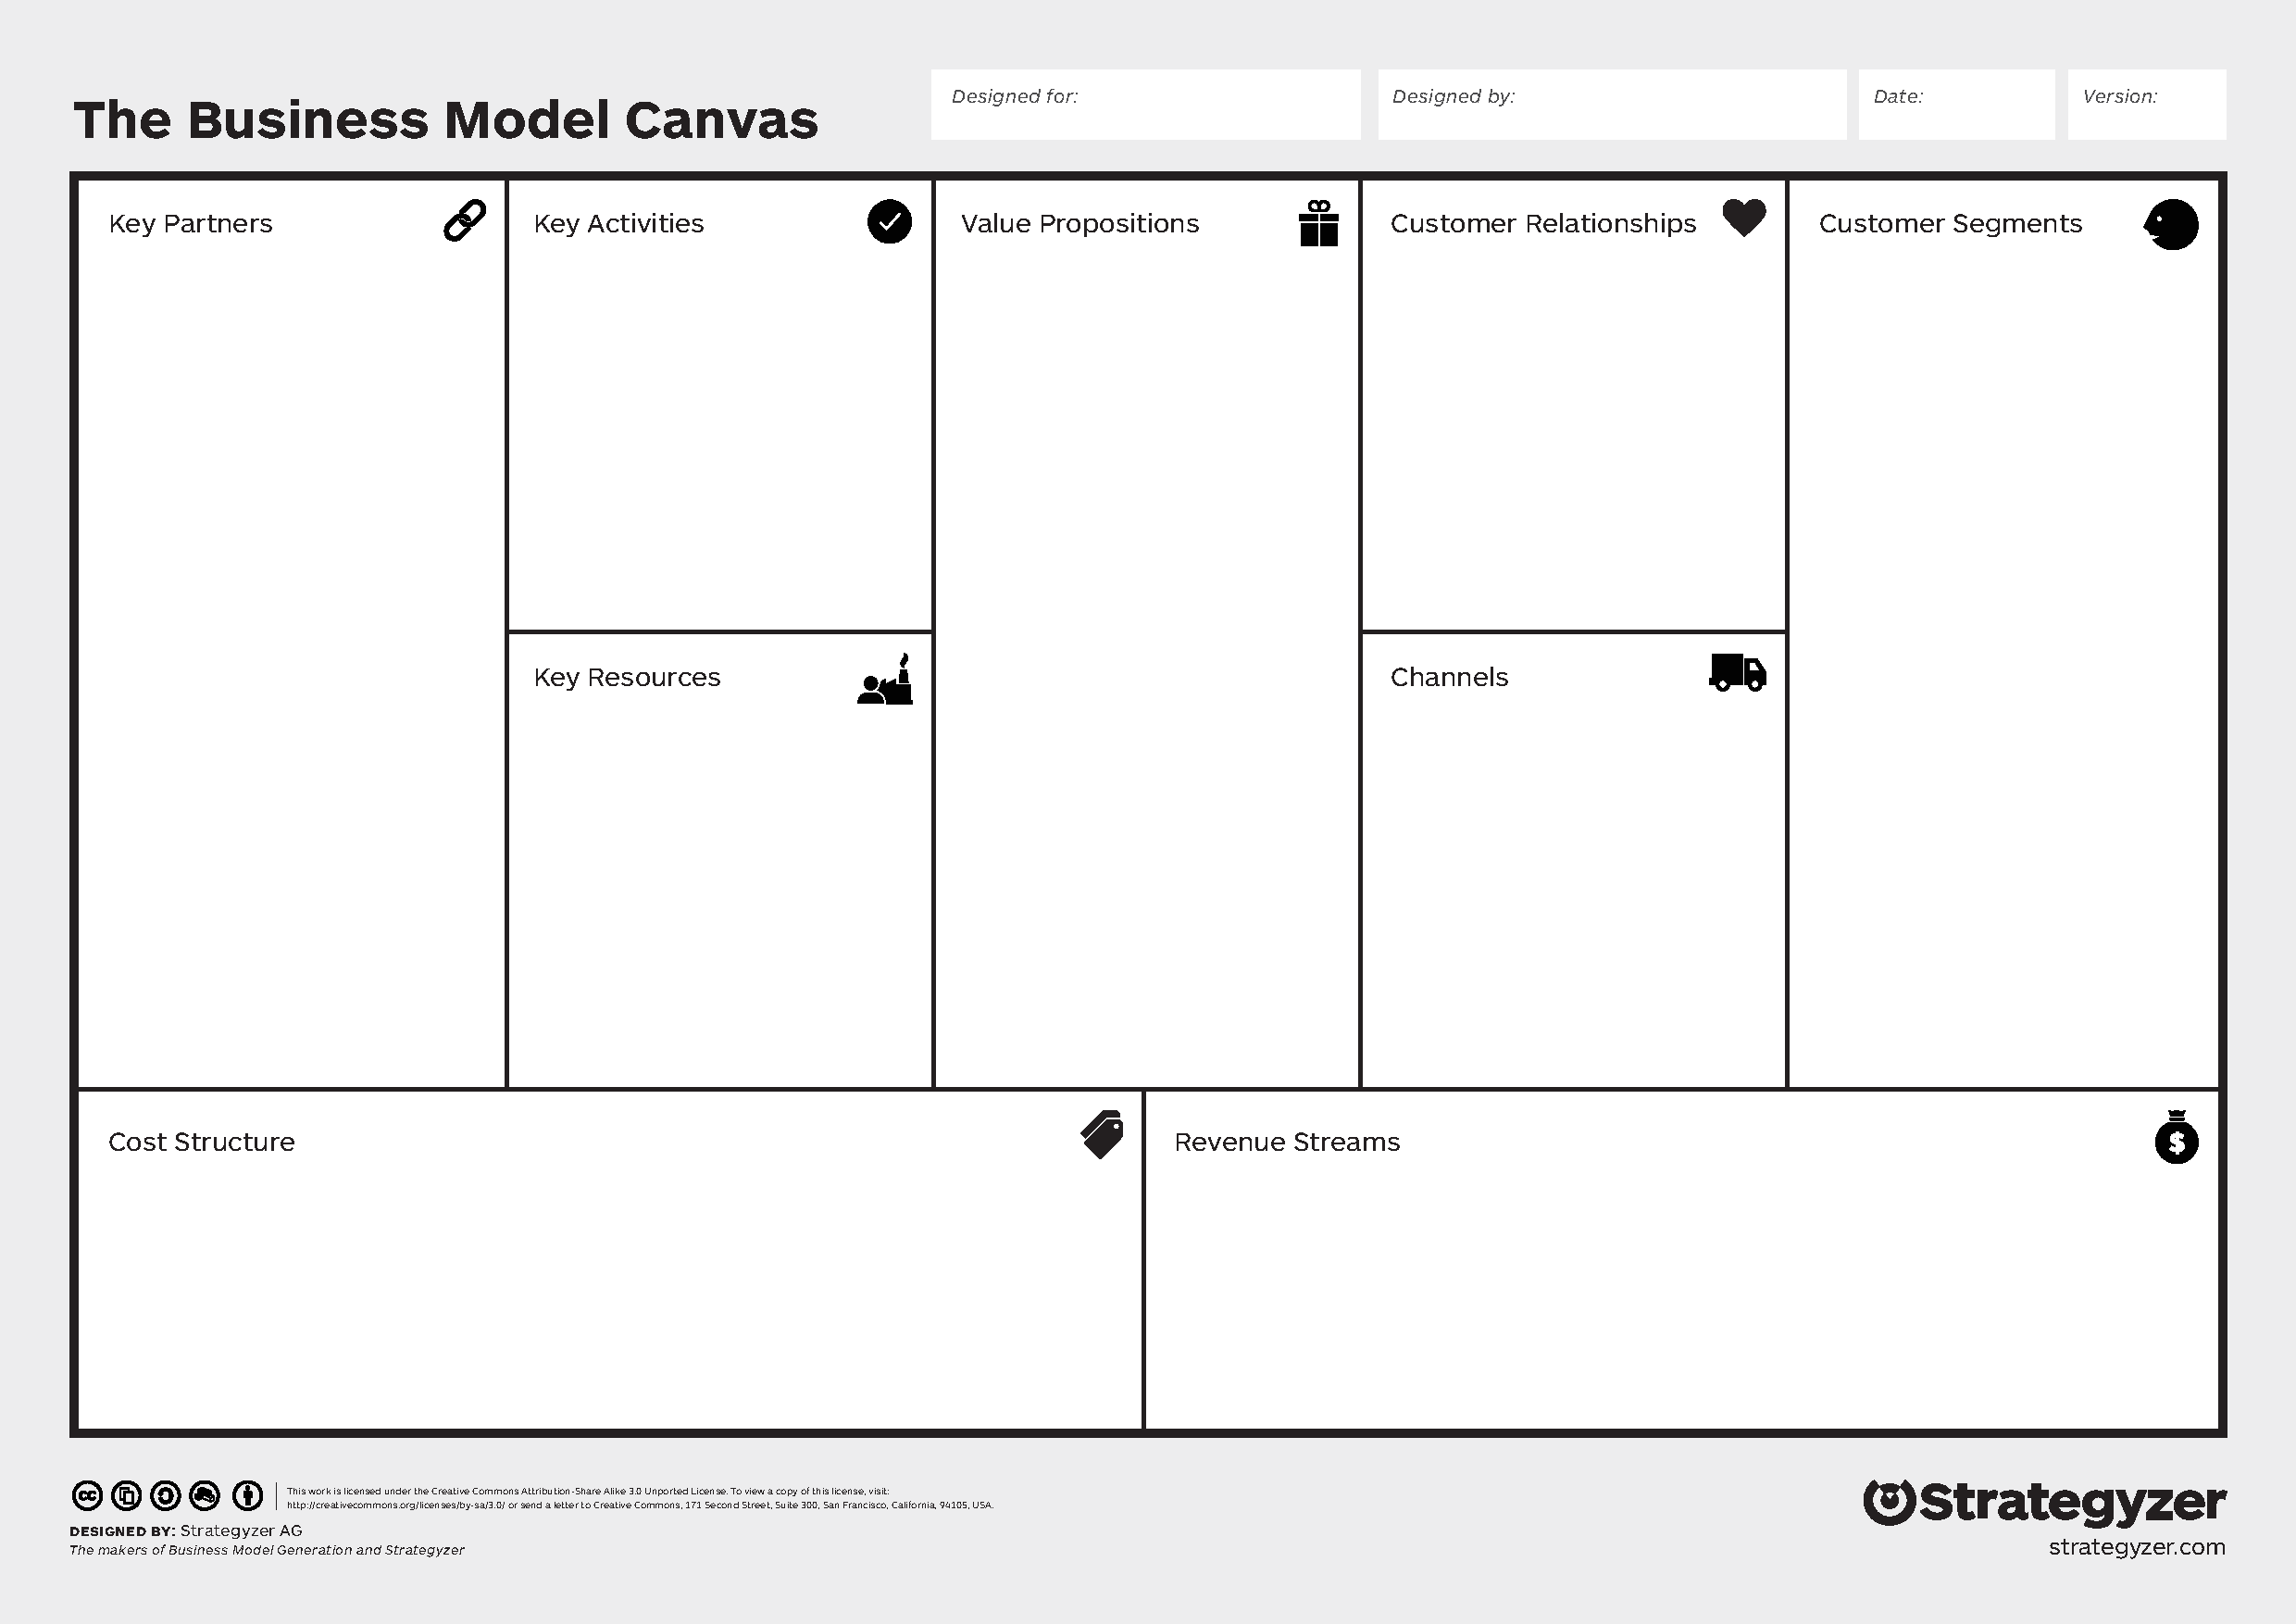
\includepdf[pages={-},landscape=true]{business-model-canvas.pdf}

\clearpage

\end{document}
